% Template for ICME-2016 paper; to be used with:
%          spconf.sty  - ICASSP/ICIP LaTeX style file, and
%          IEEEbib.bst - IEEE bibliography style file.
% --------------------------------------------------------------------------
\documentclass{article}
\usepackage{spconf,amsmath,epsfig}
\usepackage{helvet}
\usepackage{courier}
\usepackage{amsthm}
\usepackage{amssymb}
\usepackage{algorithm}
\usepackage{algpseudocode}
\usepackage{graphicx}
\pagestyle{empty}


\begin{document}\sloppy

% Example definitions.
% --------------------
\def\x{{\mathbf x}}
\def\L{{\cal L}}


% Title.
% ------
\title{Online Self-Organizing Hashing}
%
% Single address.
% ---------------
\name{Junxuan Chen, Yaoyi Li, Hongtao Lu\sthanks{Corresponding author}}

\address{Key Laboratory of Shanghai Education Commission for Intelligent Interaction and Cognitive Engineering\\
Department of Computer Science and Engineering\\	
Shanghai Jiao Tong University, P.R.China \\
chenjunxuan@sjtu.edu.cn, dsamuel@sjtu.edu.cn, htlu@sjtu.edu.cn}


%
% For example:
% ------------
%\address{School\\
%	Department\\
%	Address\\
%   Email}
%
% Two addresses (uncomment and modify for two-address case).
% ----------------------------------------------------------
%\twoauthors
%  {A. Author-one, B. Author-two\sthanks{Thanks to XYZ agency for funding.}}
%	{School A-B\\
%	Department A-B\\
%	Address A-B}
%  {C. Author-three, D. Author-four\sthanks{The fourth author performed the work
%	while at ...}}
%	{School C-D\\
%	Department C-D\\
%	Address C-D\\
%   Email}
%

\maketitle


%
\begin{abstract}
Hashing for similarity search in large scale data has become an increasingly popular technique. K-means Hashing (KMH) has been proven effective because of the benefits of adaptive k-means quantization. However, KMH is a batch-based learning model requiring high time and storage complexities, which makes it hard to load large scale data into memory to train and deal with streaming data. To address this problem, in this paper we propose an online hashing method using Self-Organizing Map (SOM) algorithm, named as Online Self-Organizing Hashing (SOH). Specifically, we map the training data to an affinity preserving hyper-cube with each vertex assigned a binary code using a SOM alike algorithm. After training, a new data point is quantized into a vertex of the hyper-cube and encoded into related binary code. Experimental results demonstrate that SOH has better or comparable retrieval performance to various state-of-the-art hashing methods while simultaneously requiring rather low computational complexity and storage space.
\end{abstract}
%
\begin{keywords}
Hashing, Self-Organizing Map, Unsupervised Learning
\end{keywords}
%
\section{Introduction}
\label{sec:intro}

The explosive growth of the vision data on the internet has posed a great challenge to many applications in terms of fast similarity search. To handle this problem, hashing based approximate nearest neighbors (ANN) search has attracted considerable attention because of their improvements in computational speed and storage reduction.

One of the most well-known data-independent hashing methods is Locality-Sensitive Hashing (LSH) \cite{gionis1999similarity}. It makes use of simple random
hyper-planes for hash functions. Following LSH, many data-dependent hashing methods \cite{gong2013iterative,wang2012semi} based on hyper-planes have
been proposed.
In these methods, several hyper-planes are generated in certain ways and partition the space into a number of non-overlapping regions in the
first stage. Then in the second stage, the data points in each region will be quantized into same binary codes.
\begin{figure}[ht]
	\vskip 0.2in
	\begin{center}
		\centerline{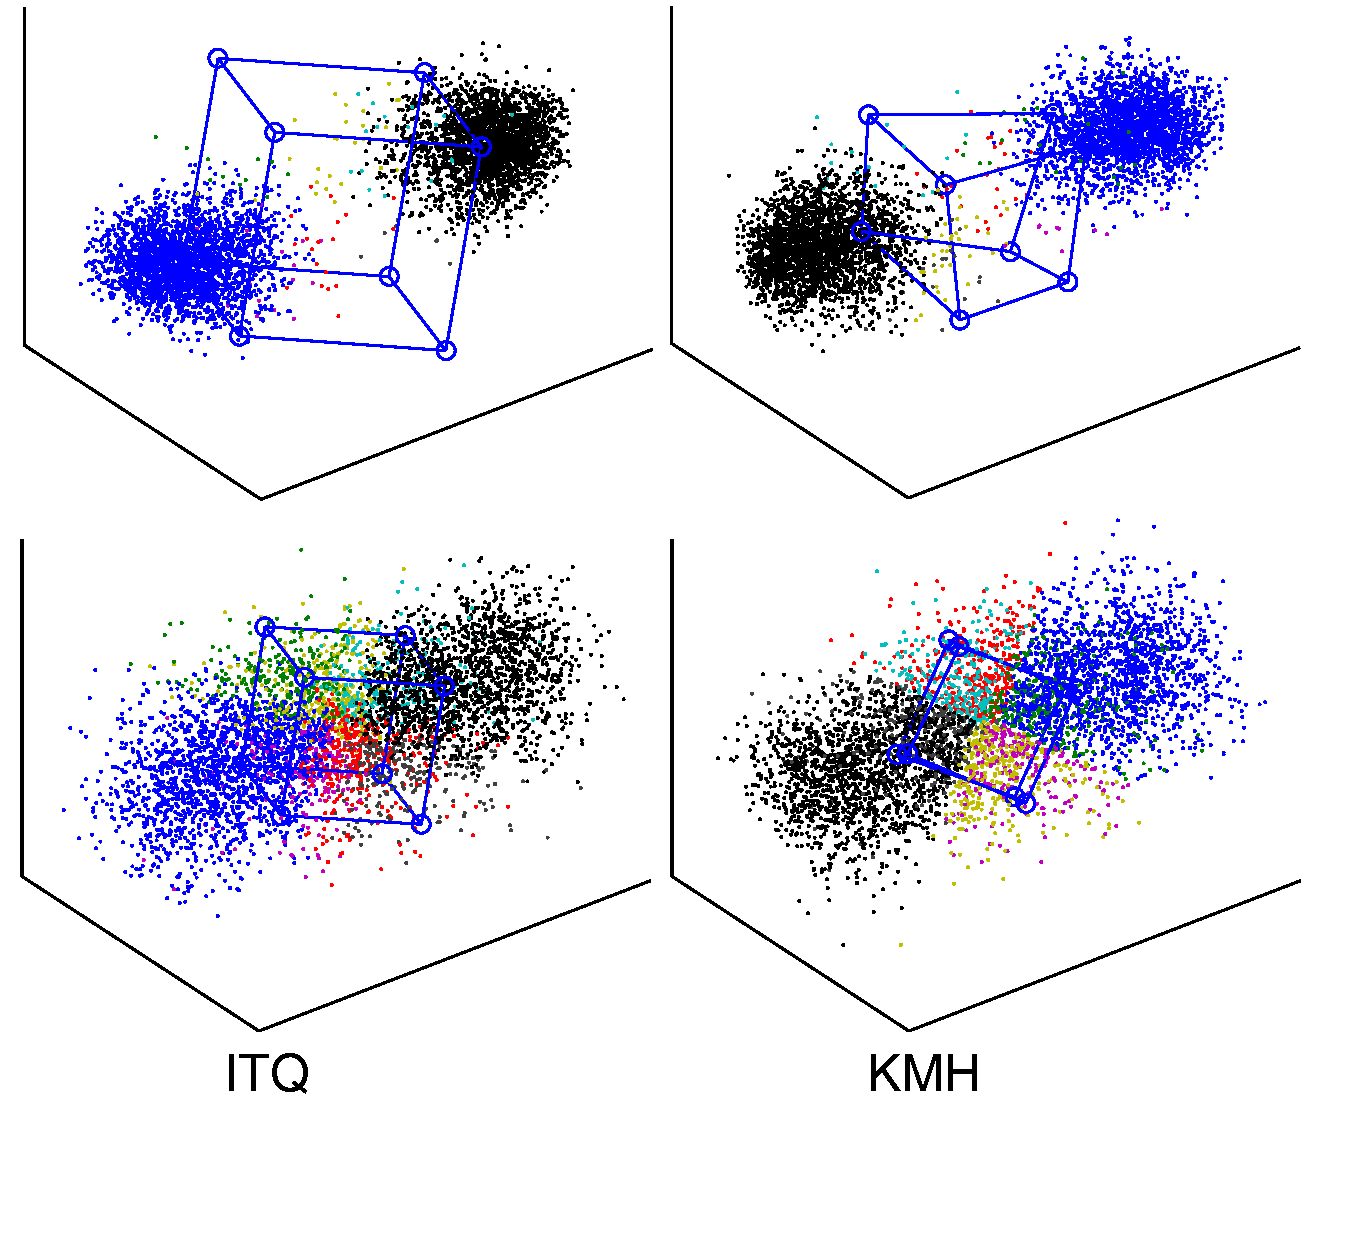
\includegraphics[width=0.76\columnwidth]{geometricview}}
		\caption{A geometric view of the hyper-cubes of ITQ and KMH on two synthetic datasets. A circle denotes a codeword, and a line
			linking two circles means their Hamming distance is 1. Data points with same indices share a same color. This figure is best viewed in color version.}
		\label{kmh_geo}
	\end{center}
	\vskip -0.2in
\end{figure}

At the same time, hashing methods like Spherical Hashing \cite{heo2012spherical} and K-means Hashing (KMH) \cite{he2013k} which do not depend on hyper-planes have been proposed.
These methods provide stronger power in defining a tighter closed region in the  data space \cite{heo2012spherical} than those using hyper-planes and achieve a promising  performance.
In KMH, a geometric view is proposed that any orthogonal hyper-planes hashing
method (\emph{e.g.}, ITQ and PCAH \cite{gong2013iterative}) can be considered as a vector quantization  using the vertexes of a rotated hyper-cube as the codewords.
KMH minimizes the sum of \emph{quantization error} and \emph{affinity error} by an Expectation-Maximization (EM) alike algorithm. Geometrically, it allows to \emph{stretch} the hyper-cube while rotating it (Figure \ref{kmh_geo}). Enjoying the benefits of adaptive k-means quantization and affinity preserving, KMH outperforms various hyper-planes based hashing methods \cite{he2013k}.

Although these hashing methods obtain good performance, however, two critical problems have been mentioned \cite{huang2013online}. First, for truly large scale datasets, data is usually stored on a distributed disk group and is too large to be read into memory. For example, KMH uses PCAH to initialize the hyper-cube which needs an infeasible time complexity of $O(nd^{2} + d^{3})$ when $n$ and $d$ are too large. Second, data points come continuously in streaming fashion in many real-word applications, while KMH has to accumulate all the data and re-train a new model.

To overcome these problems, two online hashing methods have been developed  named Online Hashing (OKH) \cite{huang2013online} and Online Sketching Hashing (OSH) \cite{leng2015online}. OKH adapts the hash function accommodate to new pair of data along the line of "Passive-Aggressive" method. OSH maintains a sketch of data that preserves the property of interest but with a smaller size and learns the hash functions based on the sketch. These methods both need one pass over data to train and allow a dramatic reduction in computation and storage. However, they are both hyper-planes based online hashing methods. As far as we know, there is no online hashing which does not depend on hyper-planes.

In this paper we focus on learning binary codes through an online affinity preserving quantization which does not depend on hyper-planes. A naive solution to the issue is  applying Stochastic Gradient Descent (SGD) to optimize the objective function of KMH. However, we find the method does not work well. This motivates us to propose a novel  Self-Organizing Hashing (SOH) based on Self-Organizing Map \cite{kohonen1998self} algorithm to optimize the joint of quantization and affinity error. Our method has two advantages:
\begin{itemize}
	\item We suppose that train samples are given one at a time. When a new sample comes we update our model immediately. It is particularly suitable
	for large scale applications, where the number of data points and the problem dimensionality are both extremely large.
	\item The topological order can be kept during iterations so it is naturally suitable for constructing a hyper-cube in feature space. Besides the superiority over hyper-planes based methods, our approach empirically possesses lower quantization error and affinity error simultaneously comparing with applying SOM algorithm or SGD directly.
\end{itemize}

To the best of our knowledge, this is  the first work that applies SOM in hashing methods. Experimental results show that our method has achieved promising performances on two large datasets.

\section{Related Work}
\subsection{K-means Hashing}
K-means Hashing is a novel affinity-preserving hashing based on k-means algorithm. Given the dataset $\mathbf{X} = [\mathbf{x}_{1}, \mathbf{x}_{2},...,\mathbf{x}_{n}]^{T} \in R^{n\times d}$ ,
KMH first constructs a set of vectors $\mathbf{W} = [\mathbf{w}_{1},  \mathbf{w}_{2}, ..., \mathbf{w}_{k}]^{T} \in R^{k\times d}$.
The set $\mathbf{W}$ is a codebook, $\mathbf{w}_{i}$ is a codeword, and each codeword has a binary indexing $\mathbf{y}_{i}\in \{0, 1\}^{b}$ with $b$ denoting the code size and $k=2^{b}$. Then KMH maps each data point $\mathbf{x}$ to a codeword $\mathbf{w}_{i(\mathbf{x})}$ and minimizes the objective function:
\begin{equation}\label{4}
E = E_{\mathrm{quan}} + \rho E_{\mathrm{aff}}.
\end{equation}
Where $E_{\mathrm{quan}}$ is the average \emph{quantization error} of the classical k-means algorithm:
\begin{equation}\label{1}
E_{\mathrm{quan}} = \frac{1}{n}\sum_{\mathbf{x}\in \mathbf{X}} ||\mathbf{x}-\mathbf{w}_{i(\mathbf{x})}||^{2},
\end{equation}
and $E_{\mathrm{aff}}$ is the \emph{affinity error} due to the distance approximation by binary code:
\begin{equation}
E_{\mathrm{aff}}= \sum_{i=1}^{k}\sum_{j=1}^{k}w_{ij}(d(\mathbf{w}_{i}, \mathbf{w}_{j}) - d_{h}(i, j))^2.
\end{equation}
Here $w_{ij} = n_{i}n_{j}/n^{2}$. $n_{i}$ and $n_{j}$ are the number of samples having index $i$ and $j$ respectively. $d_{h}$ is a Hamming-based distance between two binary indices $\mathbf{y}_{i}$ and $\mathbf{y}_{j}$:
\begin{equation}\label{d_h}
d_{h}(i,j) \triangleq s \cdot h^{\frac{1}{2}}(\mathbf{y}_{i},\mathbf{y}_{j}),
\end{equation}
where $s$ is a scale constant and initialized by PCAH, $h$ denotes the Hamming distance.
KMH minimizes this function in an EM fashion like k-means.
\subsection{Self-Organizing Map}
\begin{algorithm}[tb]
	\caption{Self-Organizing Map algorithm}
	\label{alg:som}
	\begin{algorithmic}
		\Repeat
		\State 1.At each time $t$, present an input $\mathbf{x}(t)$, and select the winner,
		\begin{equation}\label{5}
		v(t) = \mathrm{arg\ min}_{1 \leq i \leq k} || \mathbf{x}(t) - \mathbf{w}_{i}(t)||
		\end{equation}
		\State 2.Update the weights of the winner and its neighbours,
		\begin{equation}\label{6}
		\Delta\mathbf{w}_{i}(t) = \alpha(t)\eta(v, i, t)\big(\mathbf{x}(t) - \mathbf{w}_{i}(t)\big)
		\end{equation}
		\Until{converges}
	\end{algorithmic}
\end{algorithm}
Self-Organizing Map (SOM) \cite{kohonen1998self} is a powerful unsupervised neural network  for high-dimensional  data quantization
and topology preservation.

The SOM uses a set of neurons, often arranged in a 2-D rectangular 
grid, to form a discrete topological mapping of the $d$ dimensional input space  $\mathbf{X}$. Here we assume that the grid dimension is $b$ and there are $k$ neurons in the gird. So we have a set of location vector $\mathbf{R} = [\mathbf{r}_{1},  \mathbf{r}_{2}, ..., \mathbf{r}_{k}]^{T} \in R^{k\times b}$ in the grid. At the start of the learning,
all the weights $\mathbf{W} = [\mathbf{w}_{1},  \mathbf{w}_{2}, ..., \mathbf{w}_{k}]^{T} \in R^{k\times d}$ are initialized
to small random numbers, where $\mathbf{w}_{i}$ is the weight vector associated to neuron $i$ and
is a vector of the same dimension $d$ of the input $\mathbf{x}$. Then
the algorithm repeats the steps shown in Algorithm \ref{alg:som}, where $\eta(v, i, t)$ is the
neighbourhood function.
Although one can use any neighbourhood function, a Gaussian form is
often used in practice:
\begin{equation}\label{7}
\eta(v, i, t) = exp\Big(-\frac{Dist(\mathbf{r}_{v} , \mathbf{r}_{i})}{2\sigma(t)^{2}}\Big),
\end{equation}
\begin{equation}\label{8}
\sigma(t) = \sigma_{0}exp(-\frac{t}{\lambda}),
\end{equation}
The learning rate, $\alpha(t)$ in Eq.(6), is also an exponential decay function and ensures that the SOM will converge:
\begin{equation}\label{9}
\alpha(t) = \alpha_{0}exp(-\frac{t}{\lambda}),
\end{equation}
It has been shown that while SOMs with a small number of nodes behave like k-means, larger SOMs rearrange data in a way that is fundamentally  topological in character. Hence, our SOM based hashing is expected to preserve affinity better than using SGD to minimize Eq.(\ref{4}).
\section{The Proposed Approach}
\subsection{Online Self-Organizing Hashing}
Motivated by SOM, our SOH is to quantize the feature space in an \emph{online self-organizing} fashion rather than an \emph{off-line EM} fashion. Instead of using traditional 2-D or 1-D map, we construct
$b$ dimensional hyper-cube in the grid space, that is, a hyper-cube of $k=2^{b}$ points for indexing so
that each point has a $b$-bit unique binary code $\mathbf{y}_{i}$. We minimize the following affinity-preserving sample function at each step:
\begin{equation}\label{objective_soh}
\begin{split}
E(t) = \sum_{i=1}^{k} \eta(v, i, t) \big( ||\mathbf{x}(t) - \mathbf{w}_{i}||^{2} + \beta  E_{\mathrm{aff}}(\mathbf{w}_{i})\big)
\end{split}
\end{equation}
Here $\beta$ is a fixed weight and we denoting
\begin{equation}\label{E_aff_w}
E_{\mathrm{aff}}(\mathbf{w}_{i}) =  \sum_{j=1}^{k}(d(\mathbf{w}_{i}, \mathbf{w}_{j}) - d_{h}(i, j))^{2}
\end{equation}
This leads to a new update formula at  step 2 in Algorithm \ref{alg:som}:
\begin{equation}\label{eq_newupdate}
\begin{split}
\Delta\mathbf{w}_{i}(t) = &  \alpha(t)\eta(v, i, t)\big(\mathbf{x}(t) \\ &- \mathbf{w}_{i}(t) -  \beta \frac{\partial E_{\mathrm{aff}}(\mathbf{w}_{i})}{\partial \mathbf{w}_{i}}\big)
\end{split}
\end{equation}
We can derive from Eq.(\ref{E_aff_w}) that:
\begin{equation}\label{eq_partial}
\frac{\partial E_{\mathrm{aff}}}{\partial \mathbf{w}_{i}} = \sum_{j=1}^{k}4 \Big(1 - \frac{d_{h}(i, j)}{d(\mathbf{w}_{i}, \mathbf{w}_{j})} \Big)(\mathbf{w}_{i} - \mathbf{w}_{j})
\end{equation}

In each iteration we adjust the index points according to Eq.(\ref{eq_newupdate}) and Eq.(\ref{eq_partial}). We compute the
distance of two index points in Eq.(\ref{7}) in grid using the square of Hamming distance of their binary indices:
\begin{equation}\label{10}
Dist(\mathbf{r}_{v} , \mathbf{r}_{i}) = h(\mathbf{y}_{v}, \mathbf{y}_{i})^2,
\end{equation}

After learning, we assign each sample $\mathbf{x} \in \mathbf{X}$ a binary code as the binary indices of the nearest index point.
\subsection{Initialization and choosing $s$}
KMH initializes the indices using the binary codes learned by PCAH, while our SOH can get equivalent performance when we initialize the hyper-cube arbitrarily because  SOM can follow the distribution of  the data. We initialize a regular hyper-cube with each edge parallel to the axis (Figure \ref{init}).
\begin{figure}[ht]
	\begin{center}
		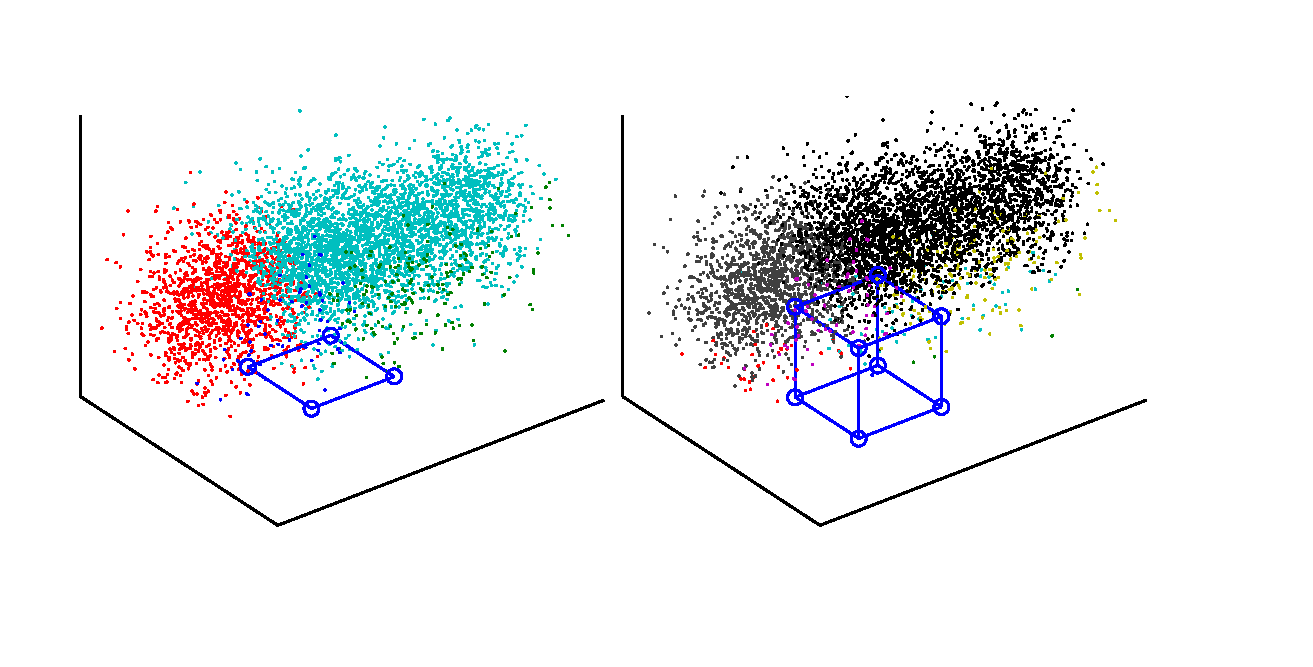
\includegraphics[width=0.76\columnwidth]{init}
		\caption{A geometric view of the initialization of SOH when feature space is 3-D, and grid space are 2-D and 3-D. Data points are synthetic and not processed with centralization.}
		\label{init}
	\end{center}
\end{figure}

We randomly initialize the scale parameter $s$ in $d_{h}(i, j)$ of Eq.(\ref{d_h}). At each iteration, before we update index points, we need to update $s$. Since Eq.(\ref{E_aff_w}) is a quadratic function of $s$ ,we have a closed form solution $\hat{s}$ :
\begin{equation}\label{optimal_s}
\hat{s} = \frac{\sum_{i}\sum_{j}d(\mathbf{w}_{i}, \mathbf{w}_{j})h^{\frac{1}{2}}(i,j)}{\sum_{i}\sum_{j}h(i,j)}
\end{equation}
The procedure of Online Self-Organizing Hashing is summarized in Algorithm \ref{alg:soh}.
\begin{algorithm}[tb]
	\caption{Online Self-Organizing Hashing}
	\label{alg:soh}
	\begin{algorithmic}
		\State Initialize the index points hyper-cube and $s$.
		\For{t = 1,2,...}
		\State 1.Update $s$ according to Eq.(\ref{optimal_s}).
		\State 2.Present an input $\mathbf{x}(t)$, and select the winner according to Eq.(\ref{5}).
		\State 3.Update the weights of the winner and its neighbours according to Eq.(\ref{eq_newupdate}) and Eq.(\ref{eq_partial}).
		\EndFor
	\end{algorithmic}
\end{algorithm}


\subsection{Generalization to a Product Space}
\begin{figure*}[t]
	\begin{center}
		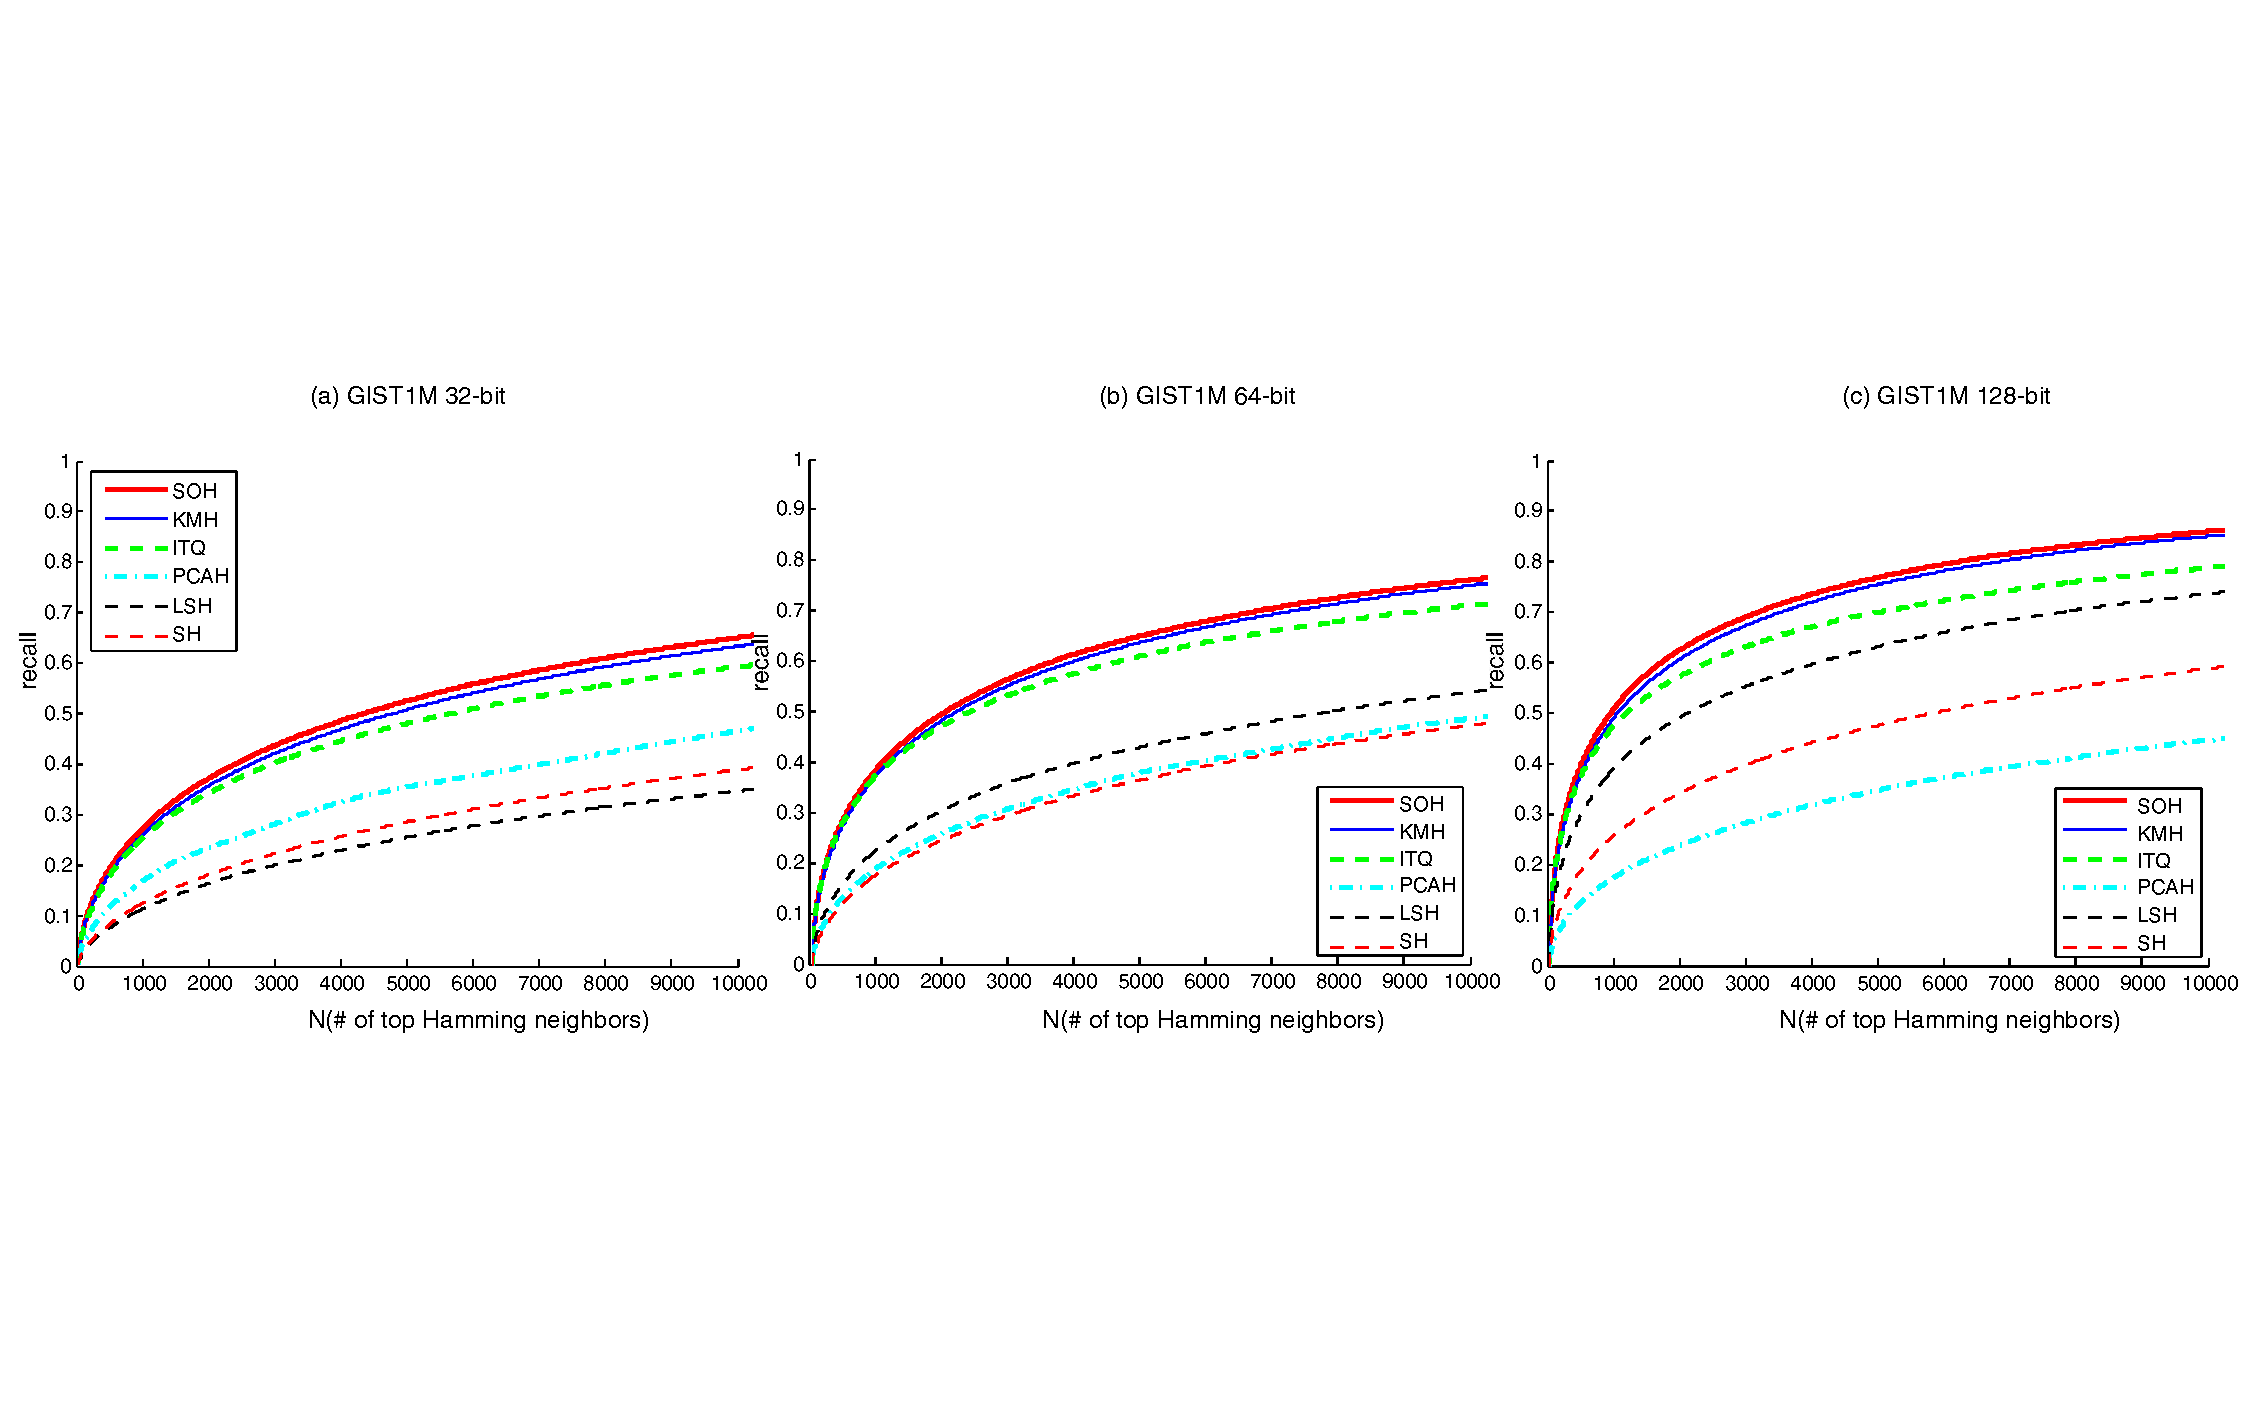
\includegraphics[width=0.92\textwidth]{batch_compare_p}
		\caption{(a)(b)(c)Recall curves on GIST1M with 32,64,128 bits. Our method and KMH uses b=4 in the 32/64-bit case, and b=8 in the 128-bit case. In this figure, K=10 Euclidean nearest neighbors are considered as the ground truth. This figure is best viewed in color version.   }
		\label{batch_compare}
	\end{center}
\end{figure*}
Like KMH, our method can be generalized to a product space in a similar way when bit number $b$ is large. We can apply random rotations to decompose the product space and get multi-table lookup as in LSH. However the retrieval performance of single hash table can not be guaranteed. To get best single hash table, we can decompose the
product space using the state-of-the-art technique Eigenvalue Allocation \cite{ge2014optimized}.
If we use Eigenvalue Allocation we need perform PCA on the dataset. We can use data sketching method \cite{leng2015online} to perform PCA in an online fashion.
In practice we find that performing online PCA on the whole dataset is unnecessary. Instead, a small subset of data is enough to generate a satisfactory decomposition before we perform our SOH.


\section{Experimental Results}
In this section, we first compare our method with applying SGD directly to optimize Eq.(\ref{4}) (we call this method KMH-SGD) to manifest the good property of SOH. Then we compare with state-of-the-art hashing methods. We conduct experiments under batch setting and online setting to verify the effectiveness and efficiency. We decompose the space to $M$ subspaces, and each sub-codebook has $b$ bits. These $M$ sub-indices are concatenated into a binary code with $M\cdot b$ bits. We control the parameter $\lambda$ to ensure the algorithm converges until each sample is presented once.
We choose $\beta = 0.5$ when $b=2$ , $\beta = 0.1$ when $b=4$ and $\beta = 0.01$ when $b=8$. Other parameters are given as $\sigma_{0} = 1$ and $\alpha_{0} = 0.05$.
\begin{figure}[t]
	\begin{center}
		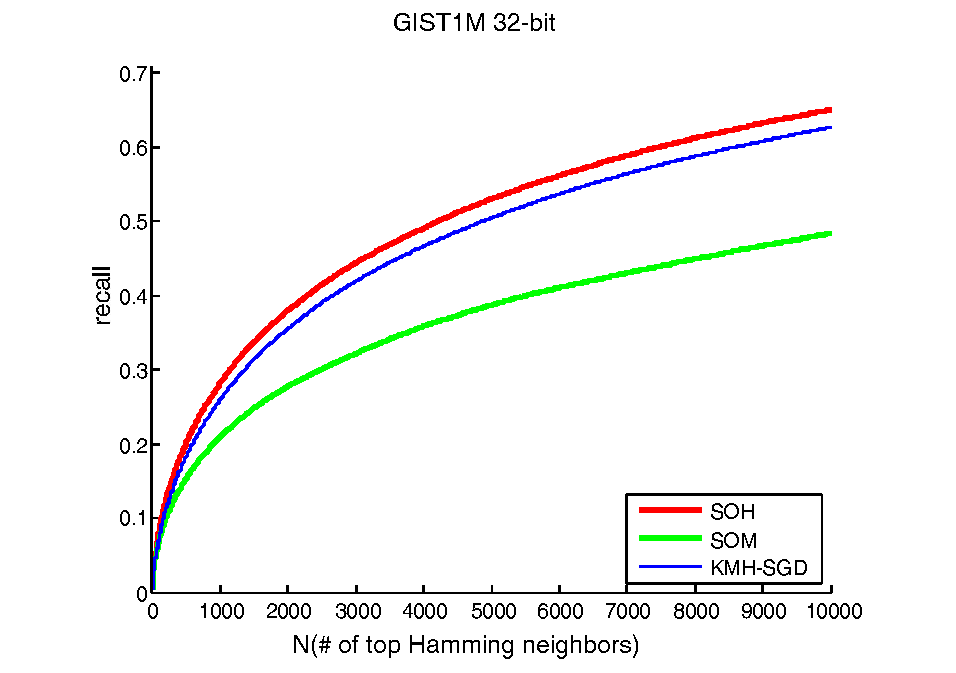
\includegraphics[width=0.76\columnwidth]{online_compare_p}
		\caption{Recall curves with three online methods on GIST1M. In this figure, K=10 Euclidean nearest neighbors are considered as the ground truth. Our method use b=4. }
		\label{somkmeans}
	\end{center}
\end{figure}
\subsection{Datasets and Evaluation Protocols}
We evaluate the retrieval performances on two public datasets: SIFT1M\footnote{http://corpus-texmex.irisa.fr} and GIST1M\footnote{http://groups.csail.mit.edu/vision/TinyImages/}.
SIFT1M contains 1 million 128-d SIFT features \cite{lowe2004distinctive} and 10,000  queries. GIST1M contains 1 million 384-d GIST features \cite{oliva2001modeling} and 10,000 independent queries randomly sampled.
For both datasets, We randomly select 100,000 data points to train under batch setting and use all data points to train under online setting.
We evaluate the performance by using each query's $K$ Euclidean neighbors in the full set of data as ground truth. In most experiments we set $K=10$ and we also evaluate the performance w.r.t a wide range of $K$. Under batch setting, we adopt \emph{Hamming ranking} to report the recall at the first $N$ Hamming neighbors. Under online setting the retrieval performance is evaluated with mean average precision (MAP). Our experiments are run on an Intel i5-4430 @ 3.0GHz CPU with 16GB RAM.
\subsection{Results and Discussions}
We first compare our method with  KMH-SGD and basic SOM algorithm without affinity preserving (Algorithm \ref{alg:som}).
\begin{figure}[t]
	\begin{center}
		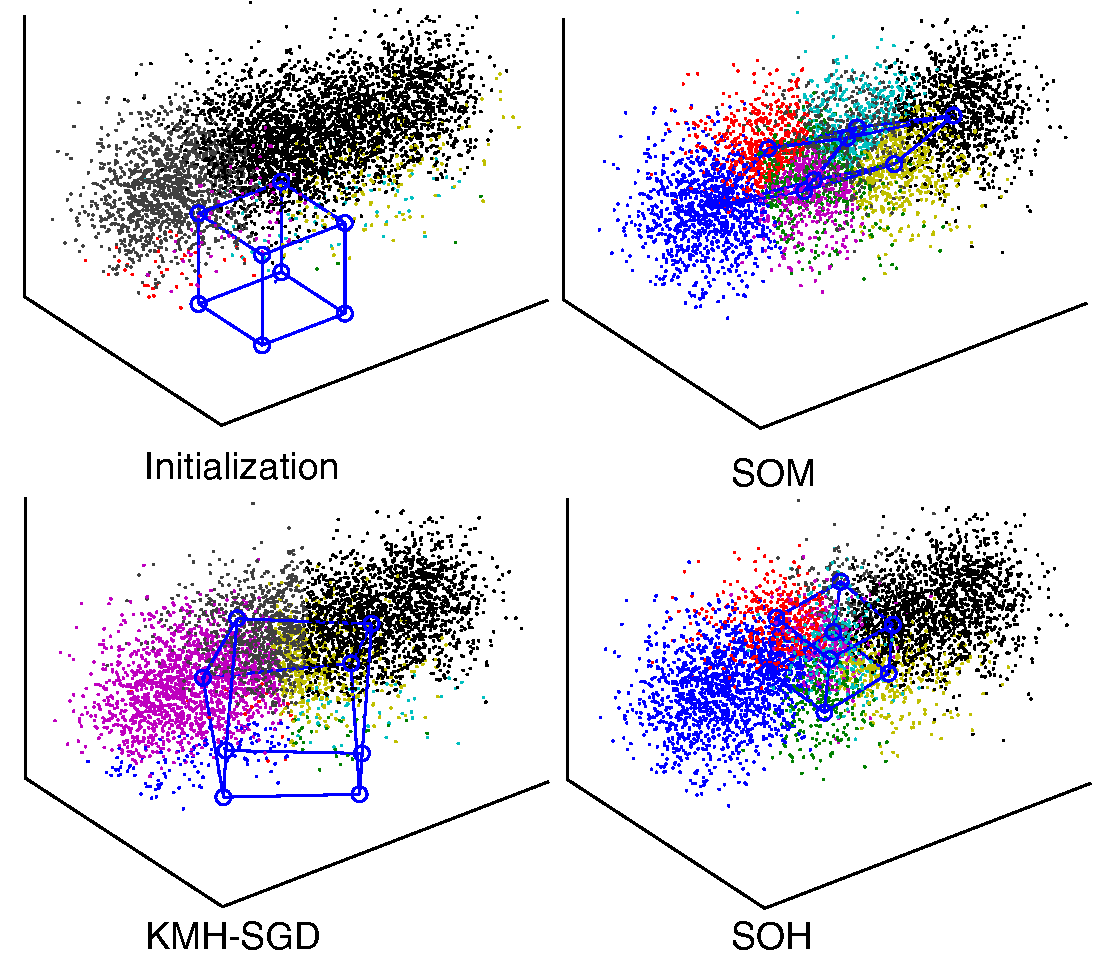
\includegraphics[width=0.76\columnwidth]{SOHvsOnlineKMS}
		\caption{A geometric view of the hyper-cubes of SOM, KMH-SGD and SOH when feature space and grid are both 3-D. Data points are synthetic and not processed with centralization. This figure is best viewed in color version.}
		\label{somall_2}
	\end{center}
\end{figure}
Figure \ref{somkmeans} shows the comparison between these methods on SIFT1M with 64 bits (M = 16 subspaces). We can see  that the basic SOM algorithm performs poorly. The KMH-SGD is better than SOM but still inferior to SOH.
To understand why these two methods is inferior,
we generate 5000 synthetic data points with non-zero mean and visualize the hyper-cube of SOM, KMH-SGD and SOH when b=3 in Figure \ref{somall_2}.
We can observe that the hyper-cube of SOM embedded into data well but collapsed when the distribution of data is not uniform. In this case, two neurons which have small Hamming distance in grid space may have large Euclidean distance in feature space, which leads to large \emph{affinity error}.
Different form SOM, KMH-SGD has considered  affinity-preserving, however, it is easier to fall into local optimum because quite a few indices will not be updated if no data point is closest to them. This situation becomes more serious when data has non-zero mean. From Figure \ref{somall_2}, we can find in this method, hyper-cube is not embedded  into  data  properly which leads to large \emph{quantization error}.
SOH has the good property of SOM and also considers affinity-preserving,  which makes it better to fit the data and has low affinity error.

Next, we compare our method with other state-of-the-art batch based hashing methods including LSH \cite{gionis1999similarity}, Spectral Hashing (SH) \cite{weiss2009spectral}, KMH \cite{he2013k}, PCAH and ITQ \cite{gong2013iterative}.  We vary hash bits from 32 to 128, and $K$ from 1 to 100 to see the performances of all methods. We present the recall curves when $K=10$ in Figure \ref{batch_compare}. It is clear that our SOH  outperforms other methods on  each bit, proving its efficiency and stability. In Figure \ref{fig_k}, we show the evaluation in a wide range of $K$ (1 to 100) comparing with KMH and ITQ. It can be seen again, our method is consistently superior.
\begin{figure}[htb]
	\begin{center}
		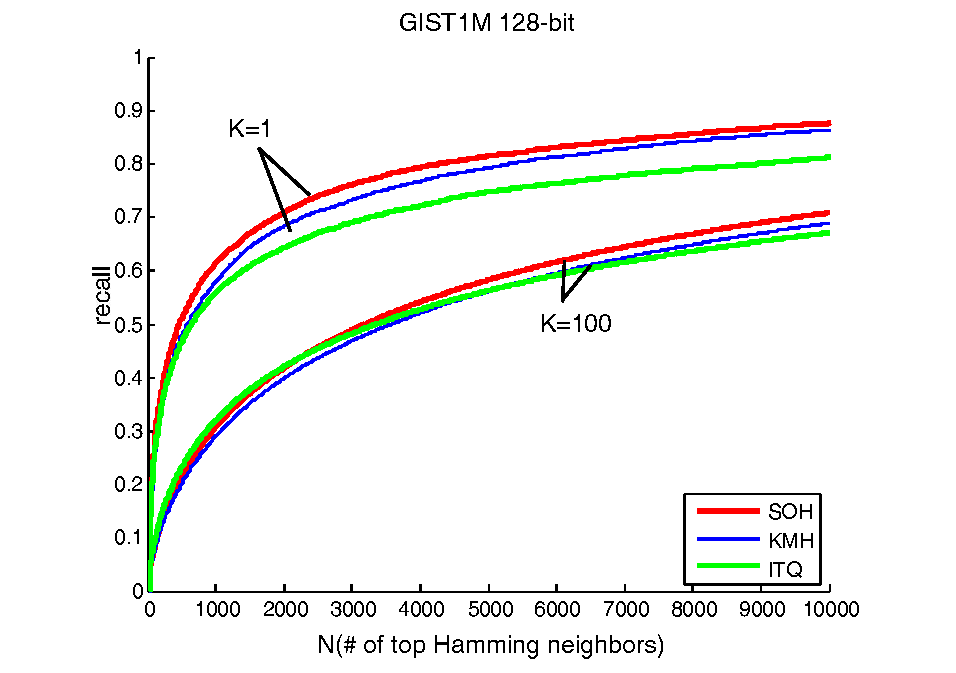
\includegraphics[width=0.76\columnwidth]{K_p}
		\caption{Comparison in GIST1M with 128 bits under different K(1, 100).}
		\label{fig_k}
	\end{center}
\end{figure}
\begin{figure*}[ht]
	\begin{center}
		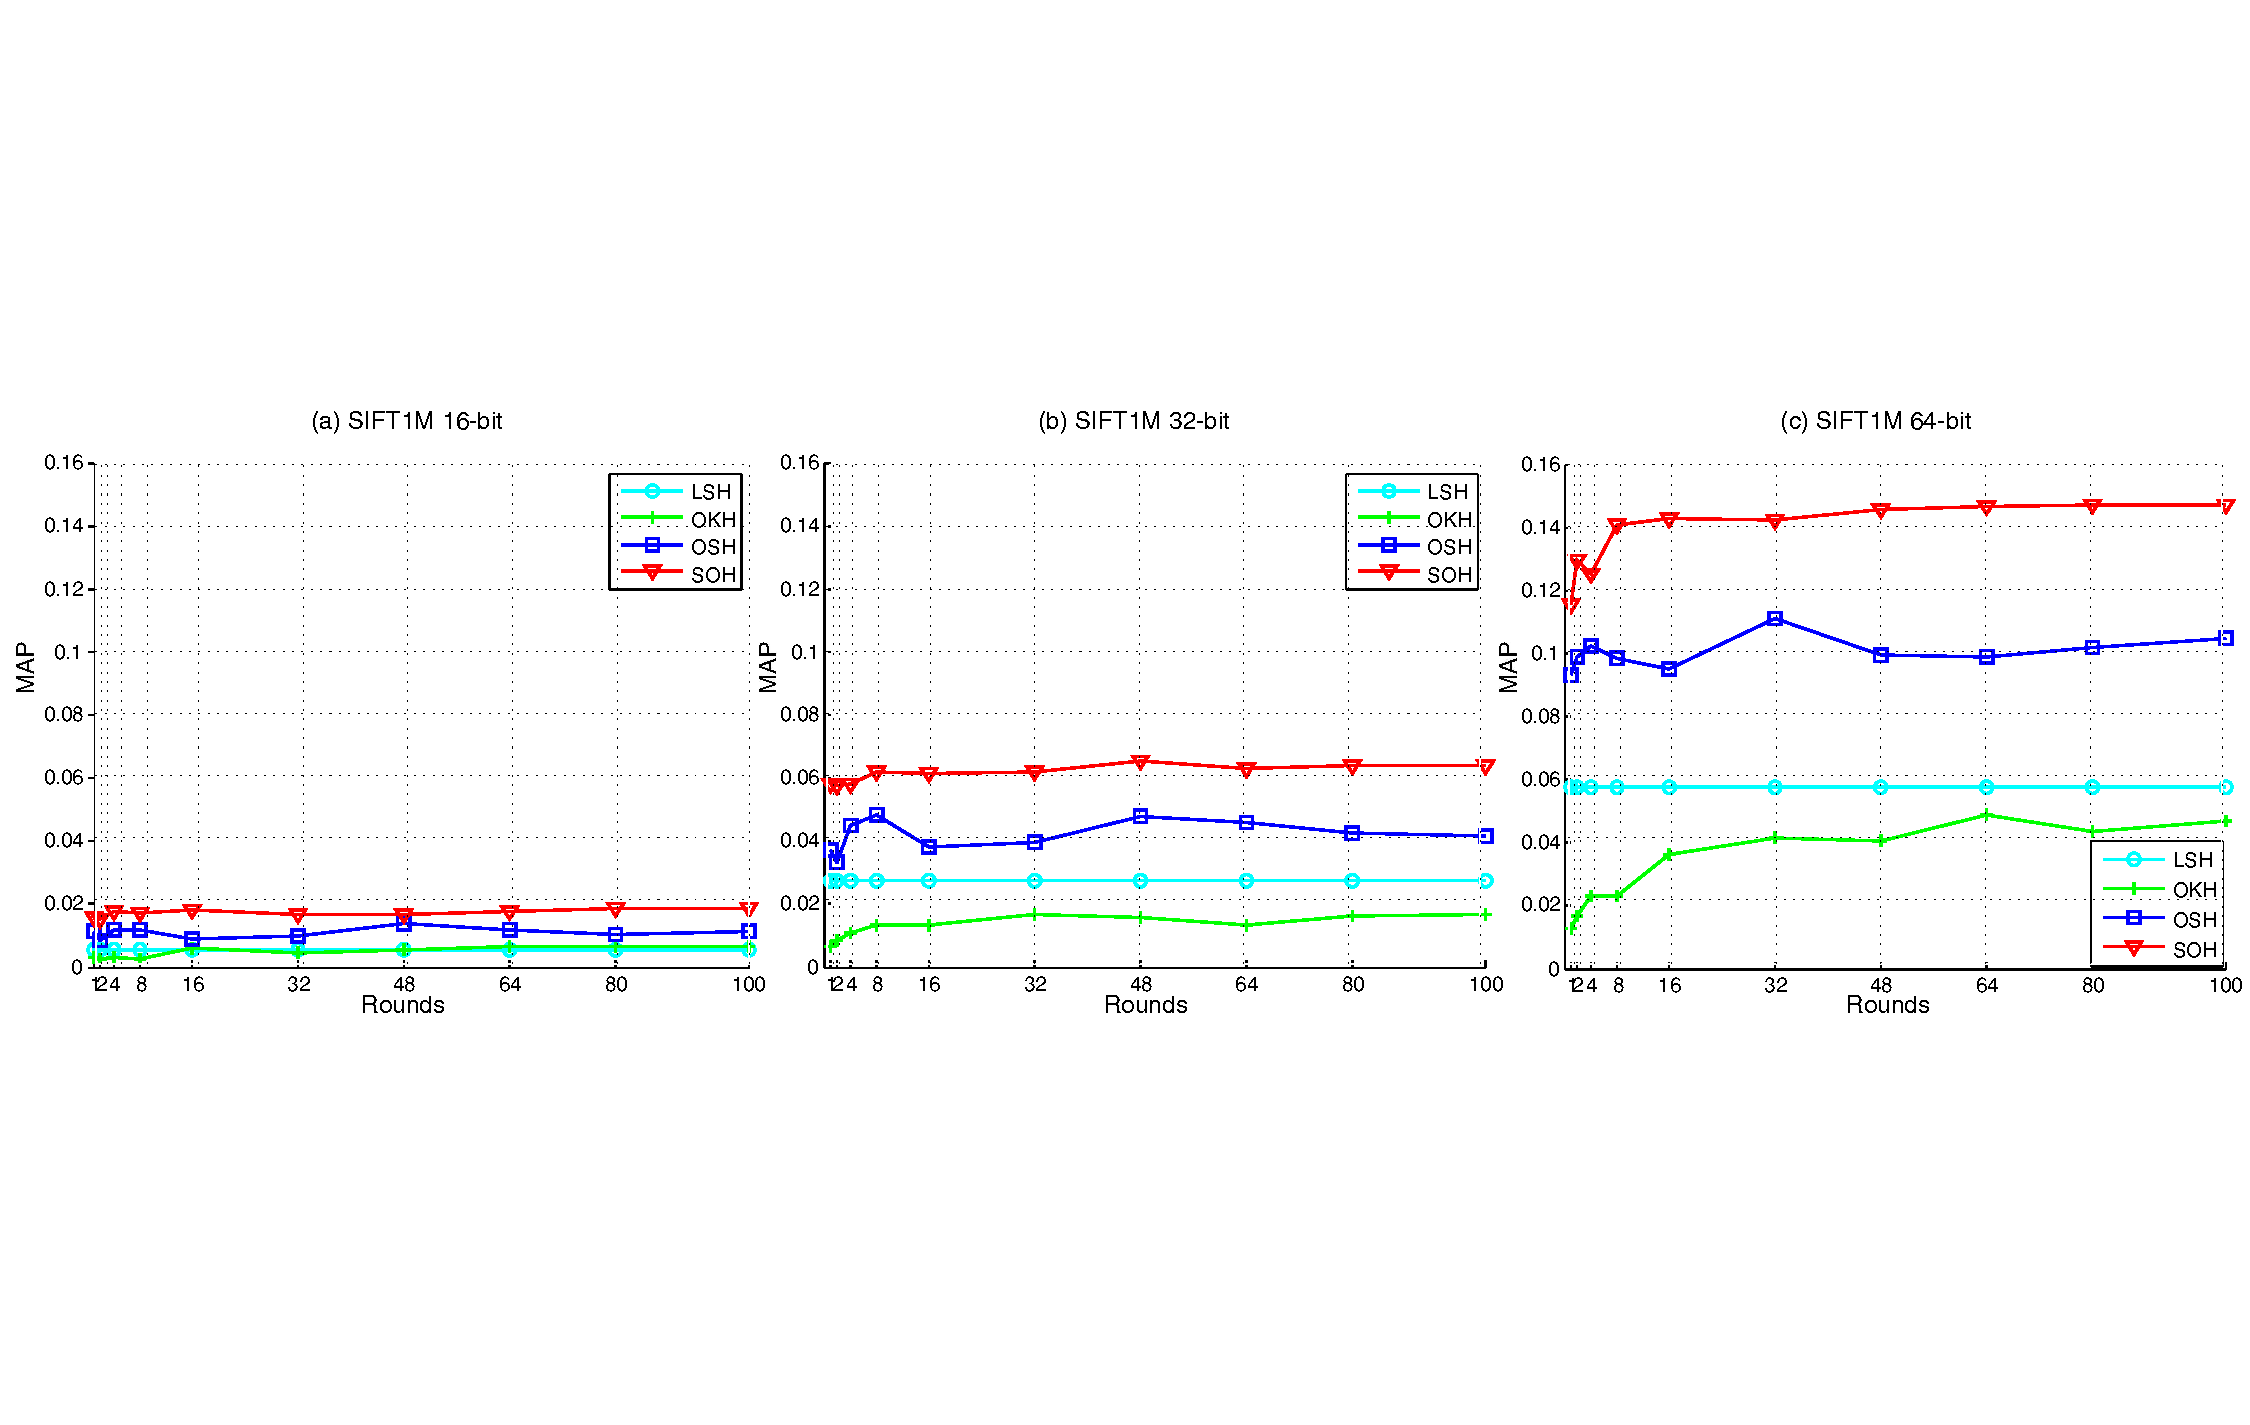
\includegraphics[width=0.92\textwidth]{onlinerst_p}
		\caption{(a)(b)(c) MAP on SIFT1M at selected rounds with 16, 32, 64 bits. Our method uses b=2 in the 16/32-bit case, and b=4 in the 64-bit case. This figure is best viewed in color version. }
		\label{compare_online}
	\end{center}
\end{figure*}

Third, for other state-of-the-art online methods, we choose OKH \cite{huang2013online}, OSH \cite{leng2015online} and LSH. For both datasets, the training data is evenly divided into 100 chunks. We evaluate the MAP scores after selected rounds. For SOH, we use 1 round (10000 points) to perform online PCA based on data sketching to decompose the space in advance.
Figure \ref{compare_online} shows the comparison between these methods on SIFT1M with 16, 32, 64 bits codes. We can observe  that SOH decisively outperforms other methods. In addition, the performance of OSH is not stable because it uses  a random rotation to the PCA projection. By contrast, SOH achieves a stably increasing accuracy in most experiments.

Finally we present the average training time of 1 round of samples (10000 points) on SIFT1M.
Although KMH performs closely to our method, it requires much more time due to the heavy iteration procedure over all data points. The comparison results with different code lengths and subspace bits are shown in Table \ref{traintime-table}. It is clear our SOH method is about 5x faster than KMH.
\begin{table}[ht]
	\caption{Training time comparison between SOH and KMH with various code length on SIFT1M (10000 points).}
	\label{traintime-table}
	\begin{center}
		\begin{small}
			\begin{sc}
				\begin{tabular}{lcccr}
					\hline
					Code length & Subspace bits & KMH(s)& SOH(s) \\
					\hline
					32    & 2 & 20.04& 5.94\\
					32    & 4 & 76.10& 7.07\\
					64    & 4 & 74.46& 14.42\\
					64    & 8 & 944.16& 152.71\\
					128   & 8 & 989.27& 241.21\\
					\hline
				\end{tabular}
			\end{sc}
		\end{small}
	\end{center}
\end{table}
\section{Conclusions and Future Work}
In this paper we proposed a novel online hashing method named Online Self-Organizing Hashing. We use classical SOM algorithm to optimize the joint of quantization error and affinity error.  Experimental
results have demonstrated our method is better or comparable to various state-of-the-art methods.
Recently, SOMs with multi-layers structures \cite{rauber2002growing,chow2006content} have been developed for image retrieval to overcome
some limitations of traditional SOM. How to integrate these works into our method seems an interesting future work.

\section{Acknowledgement}

This paper is supported by NSFC (No. 61272247, 61533012, 61472075), the 863 National High Technology Research and Development Program of China ( SS2015AA020501) and the Major Basic Research Program of Shanghai Science and Technology Committee (15JC1400103).

% References should be produced using the bibtex program from suitable
% BiBTeX files (here: strings, refs, manuals). The IEEEbib.bst bibliography
% style file from IEEE produces unsorted bibliography list.
% -------------------------------------------------------------------------
\bibliographystyle{IEEEbib}
\bibliography{camera-ready_icme2016template}

\end{document}
